\chapter{Lec 06 - Probability}

\section{Probability - terminology}
\begin{itemize}
    \item \textbf{Random variable:} a variable that can take different values randomly

    \item \textbf{Probability distribution:} a description of how likely a random variable x (or a set of random variables) is to take each of its possible states.\newline\newline
    \textbf{Discrete variables:} Probability distribution is described by a \textbf{Probability mass function}
    \begin{itemize}
        \item The domain of $P$ is the set of all possible states of x ($k$ different values).
        
        \item $\forall \, x \in \text{x} \, 0 \leq P(\text{x} = x) \leq 1$
        
        \item $\sum_{x \in \text{x}}P(x) = 1$
    \end{itemize}
    E.g. Uniform distribution $\forall \, x \in \text{x} \, P(\text{x} = x) = \frac{1}{k}$\newline\newline
    \textbf{Continuous variables:} Probability distribution is described by a \textbf{Probability Density Function} (PDF) 
    \begin{itemize}
        \item The domain of $p$ is the set of all possible states of x

        \item $\forall \, x \in \text{x}\, p(x) \geq 0$

        \item $\int p(x) dx = 1$
    \end{itemize}
    E.g. Gaussian distribution

    \item \textbf{Joint probability distribution:} Probability distribution over 2 or more variables $P(\text{x} = x, \text{y} = y)$

    \item \textbf{Gaussian distribution}: The one-dimensional Gaussian with mean $\mu$ and standard deviation $\sigma$ has the following shape:
    \[G(x) = \frac{1}{\sigma \sqrt{2\pi}}e^{-\frac{(x-\mu)^{2}}{2\sigma^{2}}}\]
    \begin{center}
        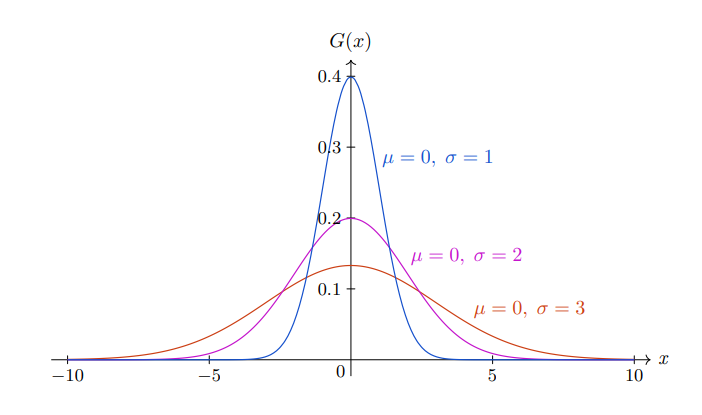
\includegraphics[]{images/Gaussian.png}
    \end{center}

    \item \textbf{Shannon Entropy (discrete variable):} 
    We can apply information theory to calculate the amount of information there is in an event. This is called \textit{self-information} and can be calculated for a \textbf{discrete} event $x$ as follows:
    \[I(x) = -log\,(P(x))\]
    where $log()$ is the base-2 logarithm and $P(x)$ is the probability of the event $x$ \footnote{other bases can be used, $e$ for example}.
    \newline\newline
    The choice of the base-2 logarithm means that the units of the information measure is in bits (binary digits). This can be directly interpreted as the number of bits required to represent an event. If the probability that an event occurs is $0.5$, we need 1 bit two represent it ($0$ fail, $1$ success); if the event occurs with probability $0.125$, we need $3$ bits to represent it (remember $y = log_a\,(x) \iff x = a^y$).
    \newline\newline
    The Shannon entropy of a \textbf{distribution} is the \textbf{expected} amount of information in an event drawn from that distribution:
    \[H(\text{x}) = - E_{x \sim P(\text{x})}[log(P(x))] = -\sum_i P(x_i) log\,P(x_i)\]
    It provides a lower bound on the number of bits needed \textbf{on average} to encode a symbol drawn from the distribution.\newline\newline
    Distributions that are nearly deterministic (where the outcome is nearly certain) have low entropy; distributions that are closer to uniform have high entropy.
    

    \item \textbf{Kullback-Leibler divergence and Cross Entropy:} Let's consider two probability distributions $P(x)$ and $Q(x)$. How can we measure how different they are?
    \begin{itemize}
        \item Kullback-Leiber divergence:
        \[D_{KL}(P \,||\, Q) = E_{x \sim P}\left[ log\frac{P(x)}{Q(x)} \right] = E_{x \sim P}[ log\, P(x) - log\, Q(x)] = \sum_i P(x_i) log\, \left(\frac{P(x_i)}{Q(x_i)}\right)\]
        It is not a true distance because it is not symmetric:
        \[D_{KL}(P \, ||\, Q) \neq D_{KL}(Q \, ||\, P)\]
        It is the measure of information lost when $Q$ is used to approximate $P$.


        \item Cross Entropy:
        \[H(P, Q) = H(P) + D_{KL}(P\, ||\, Q) = -E_{x \sim P}[log\, Q(x)]\]
        where $H(P)$ is the entropy of $P$. Note that minimizing the Cross Entropy of $P$ with respect to $Q$ is equivalent to minimize KL divergence between $P$ and $Q$. (if $P$ is given, $H(P)$ and $E_{x \sim P}[log\, P(x)]$ are constants). If $P$ is a fixed distribution minimize KL divergence or minimize CE is the same, but CE is easier to compute.
    \end{itemize}

    \item \textbf{Maximum likelihood estimation:} Is a principled way to derive estimators (models). Consider $n$ examples $Tr = \{\textbf{x}^{1}, ..., \textbf{x}^{n}\}$ drawn i.i.d. from $p_{data}$ (which is not known in advance). With machine learning we want to estimate this probability $p_{data}$ with some models that depend on a set of parameters $\theta$.\newline\newline
    Let's consider a family of parametric probability distributions (models) $p_{model}(\textbf{x}; \theta)$. It maps a point $\textbf{x}$ to a real number, estimating $p_{data} (\textbf{x})$. How can we find $\theta$ in such a way that $p_{model}$ and $p_{data}$ are as close as possible ? A possible formalization of this problem is given by the Maximum Likelihood estimation for $\theta$:
    \[\theta_{ML} = argmax_{\theta}\, p_{model}(Tr; \theta) = argmax_{\theta}\prod_{i = 1}^{n}p_{model}(\textbf{x}^{i}; \theta)\]
    Basically, we choose the probability distribution which is most likely to have produced our data. Note that we are assuming that all the examples are \textbf{independent} each other ($P(x, y) = P(x)P(y)$).
\end{itemize}

\section{Maximum likelihood}
Maximum likelihood (ML) is a special case of \textbf{maximum a posteriori estimation (MAP)}.
\[h_{MAP} = argmax_{h \in H}P(h|D)\]
\[= argmax_{h \in H}\frac{P(D|h)P(h)}{P(D)}\]
where:
\begin{itemize}
    \item $P(h):$ a priori probability of the hypothesis $h$
    \item $P(D):$ a priori probability of training data. It is the probability to observe exactly this training set when we don't know anything about the hypothesis.
    \item $P(h|D):$ probability of $h$ given $D$. It is the probability that $h$ is the hypothesis that generates data $D$.
    \item $P(D|h):$ probability if $D$ given $h$. Given a hypothesis $h$, it is the probability of data $D$ to be generated by $h$.
\end{itemize}
Since $P(D)$ does not depend on $h$, we can consider it as a constant and remove it from the equation.
\[= argmax_{h \in H}P(D|h)P(h)\]
If we assume uniform probabilities on the hypotheses, that is $P(h_{i}) = P(h_{j})$, we can choose the so called \textbf{maximum likelihood hypothesis} $h_{ML}:$
\[h_{ML} = argmax_{h \in H}P(D|h)\]
MAP and maximum likelihood approach make predictions using a single point estimate of $\theta$. The Bayesian approach is to make predictions using a full probability distribution over $\theta$. For example, given a new instance $\textbf{x}$, which is the most likely \textbf{classification}? The classification given by the most likely hypothesis $h_{MAP}$ is not necessarily the most likely classification. For example, given the following three possible hypothesis:
 \[P(h_{1} | D) = 0.4 \quad P(h_{2} | D) = 0.3 \quad P(h_{3} | D) = 0.3\]
 We want to classify a new instance $\textbf{x}$:
 \[h_{1}(\textbf{x}) = + \quad h_{2}(\textbf{x}) = - \quad h_{1}(\textbf{x}) = -\]
 The most likely hypothesis $h_{1}$ classifies $\textbf{x}$ with the label (+), but the most likely classification is (-). This is because the optimal (Bayes) classification of a certain instance is the class $v_{j} \in V$ which maximizes the following probability:
 \[argmax_{v_{j} \in V} = \sum_{h_{i} \in H}P(v_{j} | h_{i})P(h_{i} | D)\]
 where $V$ is the set of possible labels.\newline\newline
 However, in real-world problems having the probabilities $P(h_{i} | D)$ is almost impossible. Therefore, we usually make the assumption of considering the classification made by $h_{map}$ as most probable.

 \subsection{Maximum likelihood estimation}
 As we said before, the maximum likelihood estimation is defined as follows:
 \[\theta_{ML} = argmax_{\theta}\, p_{model}(Tr; \theta) = argmax_{\theta}\prod_{i = 1}^{n}p_{model}(\textbf{x}^{i}; \theta)\]
 However, computing the product of many probability is unstable. Therefore, we can apply the $log$ and the $argmax$ does not change (log-likelihood).
 \[\theta_{ML} = log(argmax_{\theta}\prod_{i=1}^{n}p_{model}(\textbf{x}^{(i)}; \theta))\]
 \[= argmax_{\theta}\sum_{i = 1}^{n}log\, p_{model}(\textbf{x}^{(i)}, \theta)\]
 We can equivalently divide by $n$ to express maximum likelihood as an expectation over training data:
 \[\theta_{ML} = argmax_{\theta}E_{x \sim \hat{p}_{data}}[log \, p_{model}(x; \theta)]\]
where $\hat{p}_{data}$ is an empirical discrete distribution that we get over the examples in the training set. This implies that maximum likelihood minimizes the dissimilarity between $\hat{p}_{data}$ and $p_{model}$, measured by the KL divergence. It also corresponds to minimize the \textbf{cross-entropy} between the two distributions.

\subsection{Conditional log likelihood}
We can use maximum likelihood to estimate a \textbf{conditional} probability $P(\textbf{y} | \textbf{x}; \theta)$ to predict $\textbf{y}$ given $\textbf{x}$ (supervised learning).
\[\theta_{ML} = argmax_{\theta} P(\textbf{Y} | \textbf{X}; \theta)\]
If input examples are i.i.d.
\[\theta_{ML} = argmax_{\theta}\sum_{i=1}^{n}log\, P(\textbf{y}^{(i)} | \textbf{x}^{(i)}; \theta)\]
Consider any real-valued target function $f$ and learning examples $\langle 
 \textbf{x}_{i}, d_{i}\rangle$ where $d_{i}$ has some noise:
 \begin{itemize}
     \item $d_{i} = f(\textbf{x}_{i}) + e_{i}$
     \item $e_{i}$ is a random variable (noise) extracted independently, for each $\textbf{x}_{i}$, according to a Gaussian distribution with mean 0.
 \end{itemize}
 It can be shown that the maximum likelihood hypothesis is the one that minimizes the mean squared error:
 \[\theta_{ML} = argmin_{\theta} \sum_{i=0}^{m}(d_{i} - \hat{y}_{i})^{2}\]
maximizing the log-likelihood with respect to $\theta$ yields the same estimate of the parameters $\theta$ as does minimizing the mean squared error.
